\documentclass[12pt]{article}
\usepackage[top=1in, right=1in, bottom=1in, left=1in]{geometry}
\usepackage{amsfonts}
\usepackage{graphicx}
\usepackage{apacite}
\usepackage{enumerate}
\usepackage{multicol}
\usepackage{amsmath}
\usepackage{subcaption}
\usepackage{listings}
\usepackage{algpseudocode}
\usepackage{algorithm}
\begin{document}
	\begin{center}
	\scalebox{2}{\fontsize{32pt}{10pt}\selectfont {Flood alert application}}\\ 
	\scalebox{2}{\fontsize{32pt}{10pt}\selectfont {using android}}
	\\[2in]
		\begin{LARGE}
		Rohit Iyer (510516084)\\
		Parnavi Sen (510516011)\\
		Sukrita Saha (510516082)\\
		Mamon Almas (510516015)\\		
		under the supervision of\\[1cm]
		Prof. Ashish Kumar Layek\\[1in]
		Department of Computer Science and Technology\\
		IIEST, Shibpur\\
		April 25, 2020\\
		\end{LARGE}
	\newpage
	\end{center}
	
	\begin{center}
	\scalebox{1}{\fontsize{32pt}{10pt}\selectfont \textbf{Abstract}}\\[1in]
In this report we develop an android application which provides real time updates and prompt flow of authentic information of flood ravaged areas to the public. The application would take as input the sets of images belonging to flood affected areas from rescue personnels, authenticate and filter them using deep learning approaches. The severity of floods is estimated and plotted on a map using the geolocations of the images. The data is analyzed by using clustering techniques and visualized on the map. Subsequently the affected areas and their peripheries are discovered for immediate relief operations.
	\end{center}\newpage
\tableofcontents
\newpage
\listoffigures
\newpage
\section{Introduction}
Extreme climate changes have become the new norm. Disaster events and their scale continue to increase. Therefore, it has become imperative to devise a quick disaster response system for minimising the magnitude of damage and reducing the casualties. The cases of flood related disasters have drastically increased especially in India with a dense population in coastal areas where the destruction due to cyclones are massive.\\\\
The Arabian sea is heating up leading to increase in cyclonic activity in the area and thus causing mayhem in the west coast. On the east coast as well, a number of natural disasters have occurred of great proportions . Recent disasters such as cyclone Aila in 2009, cyclone Fani in 2019, cyclone Amphan in 2020, cyclone Nisarga in 2020 and many more have shown how man is helpless when nature’s fury has its own say.\\\\
Four states - Andhra Pradesh, Odisha, Tamil Nadu and West Bengal and one Union Territory - Pondicherry on the East Coast are most vulnerable to cyclone disasters. An analysis of the frequencies of cyclones on the East and West coasts of India during 1891-2000 show that nearly 308 cyclones (out of which 103 were severe) affected the East coast. During the same period, 48 tropical cyclones crossed the West coast, of which 24 were severe cyclonic storms.\\[0.5cm]
Other than cyclones, monsoonal floods cause mayhem as well, with commuters getting stuck in waterlogged streets, open wires electrifying nescient citizens, loss of livelihood and shelters, etc . 
\subsection{Motivation}
Destruction due to floods can only be mitigated by immediate response to crisis situations.\\
Civic volunteers and NDRF personnels (fondly called the Rescuers) are those warriors who tackle such grave situations and provide a helping hand to the victims of the afflicted.Their work and their contribution to the society is unparalleled.\\\\
In this age of technology, if we are able to integrate such disaster response systems with cutting edge technology, we would be better equipped to handle crises. With the support of digital platforms, the information can be quickly communicated to disaster management teams about the severity of inundation.
\subsection{Proposed method}
The aim was to create an application which would be helpful for smooth flow of relevant information and subsequently result in swift actions at the eventuality of a flood related disaster.\\
This application would be useful for the general public as they would be promptly notified of the flood affected zones in their respective cities and where they should not be venturing out. \\\\
Key features of the flood alert application:
\begin{itemize}
	\item Takes images of affected locations from relief workers.
	\item Authenticates and filters flood images using an AI model.	
	\item Detects the clusters and hotspots that have suffered havoc by the floods
	\item Maps the periphery of the areas that should be avoided by the people and which needs relief aid by NDRF and civic volunteers
\end{itemize}
The civic volunteers and NDRF officials would play a major role in this transfer of real time information by uploading images of the inundated localities in different pockets of the city to the flood alert application. This would facilitate citizens to be aware of the latest developments.\\\\
Social media images are a valuable source of information and have been used in building such disaster mitigation applications previously. However, they lack important information and are also of lesser resolution. The geolocation from the metadata of images are stripped off which makes it difficult for accurate mapping of flood affected areas. Moreover, there might be too many farce images which might be of a different location or of a different date leading to inconsistencies and  delays in the hazard mitigation process.\\\\
The application extracts geolocation from metadata of the images instead of using the location from which the images are uploaded. This is beneficial in case there is poor internet supply in the affected areas and the civic volunteers choose to upload images from an unaffected area with better internet coverage.
\subsubsection{Authentication}
We found out that several images that are posted by news agencies or in social media do not actually convey any pictorial information about the said event. In flood related disasters, several images are circulated over the internet. However only half the number of images are actually relevant to the event.\\\\
Thus, these images, once having been uploaded to the server undergo a verification process. The server checks the validity of the images as to whether it belongs to the city as has been specified by the user who has pushed the image to the server.\\\\
Another layer of check is done where the image is passed through a machine learning model which authenticates the images. Only those images are allowed to be uploaded which are successfully authenticated as flood affected regions.\\\\
If an image is found to be a flood water image, it can be classified on the basis of the amount of affected portion within the image. The basic assumption we take is that the severity of the flood is proportional to the amount of flood water present in the image.
This model may filter a small percentage of the relevant images as well, as per its discretion. However this loss of authentic data needs to be accepted considering that all the uploaded images allowed to be viewed by the public conveys the actual severity of floods.\\\\
Several binary CNN models were prepared by us of which the model with the pretrained weights of the state of the art VGG19 model worked pretty well. We trained the model based on our own dataset prepared by web scraping flood and non - flood images.
	\begin{figure}[h!]
		\begin{center}
		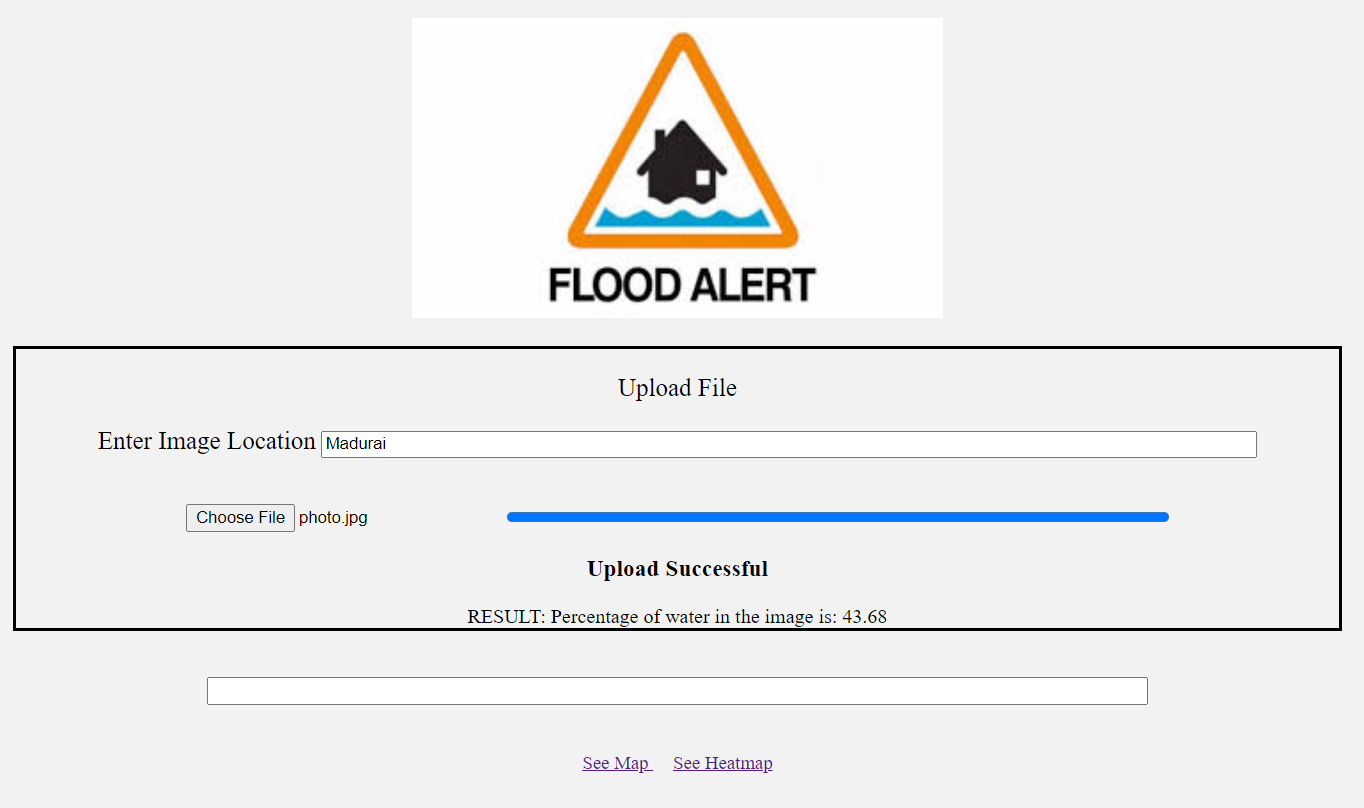
\includegraphics[width=4in]{Capture_upload.png}
		\end{center}
	\caption{Image uploaded undergoing authentication}
	\end{figure}
\subsubsection{Analytics}
The application enables the user to view the clusters of affected zones in his/her city and thus avoid travel there. The heatmap of affected regions is available to the general users to understand the severity or intensity of the catastrophe. \\
One would also be able to quickly glance through the names of the zones or districts severely afflicted. This quick flow of verified information would serve as a boon to the oblivious citizens.
\subsubsection{Mapping peripheries}
With the help of such a quick and responsive application local authorities can use it to their advantage and cordon of these “hotspots” and debar the public from venturing into the area.\\\\
Delineation of flood risk hotspots is a very challenging task for the authorities which we have automated. The detailed boundary can be used as a reference by civic authorities, power department,municipal corporation and other local authorities that need to provide urgent relief aid to the affected people.\\
It is important to underline the delineation carried out cannot replace a comprehensive evaluation by experts.
\subsubsection{Usefulness}
After the application is fully deployed, the data it gathers over a period of time can be analyzed to ascertain potential flood prone areas. Mapping the regions requiring robust infrastructure, road maintenance, location of storm water pumping stations and water tank facilities would become a tad easier for the municipal corporation. \\\\
This application can be used by the National Disaster Relief Force (NDRF) and other rescue personnel and volunteers for early detection of flood affected areas and providing urgent relief aids to the affected.\\\\
The ease of use, responsive nature and prompt flow of real time information directly from the men on ground providing relief work and subsequent analysis of the data for visualisation makes the application unique and highly beneficial. 
\section{System design}
	
	\begin{figure}[h!]
		\begin{center}
		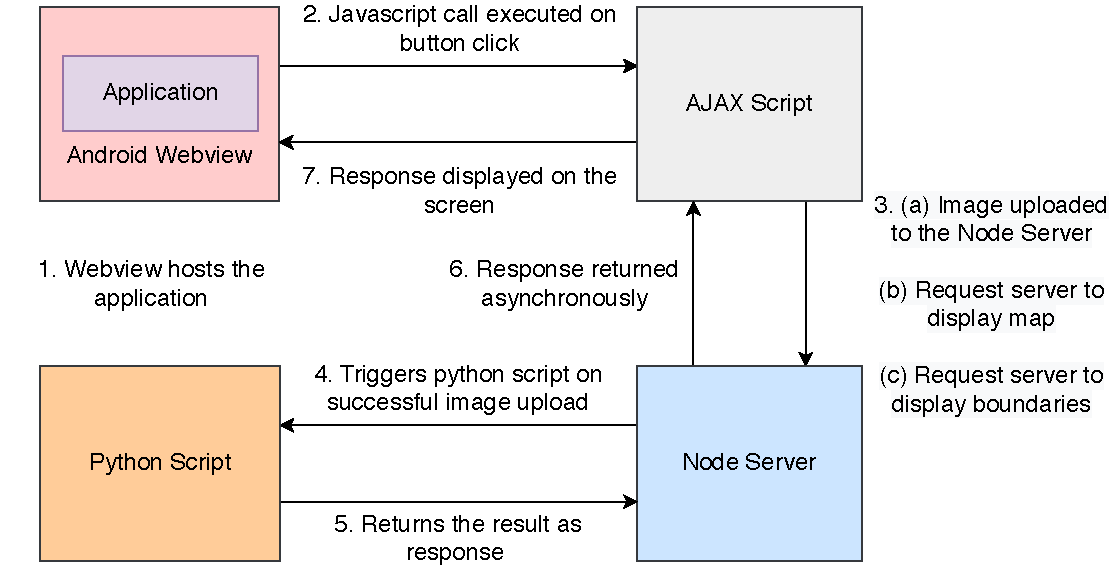
\includegraphics[width=4in]{System Design.jpg}
		\end{center}
	\caption{System Design}
	\end{figure}
	
\subsection{Framework}
	\begin{itemize}
	\item Android webview hosts the html form.
	\item Javascript call executed on button click.
	\item Server script spawns a child process.
	\item Python code executed in the backend.
	\item Backend code accesses the server database.
	\item Returns required data in JSON format.	
	\end{itemize}
\subsection{Multiple requests}
Node.js runs in a single thread. However, we can take advantage of multiple processes.\\
The spawn method spawns an external application in a new process and returns a streaming interface for I/O . spawn returns a ChildProcess object:\\\\
const \{spawn\} = require ('child\_process');\\
const child = spawn('python',["code.py", arguments]);\\\\
We can pass arguments to the command executed by the spawn as an array using its second argument.Child processes have three standard IO streams available: stdin (writeable), stdout (readable) and stderr (readable). 
On readable streams there is data event emitted when a command runs inside a child process outputs something. In this way we can send the data from the server to the client side script.\\
In our code, we passed the executable python file as argument to the spawn method which runs in the backend and provides the output.
As spawn returns a stream based object, it’s great for handling applications that produce large amounts of data.\\

	\begin{figure}[h!]
		\begin{center}
		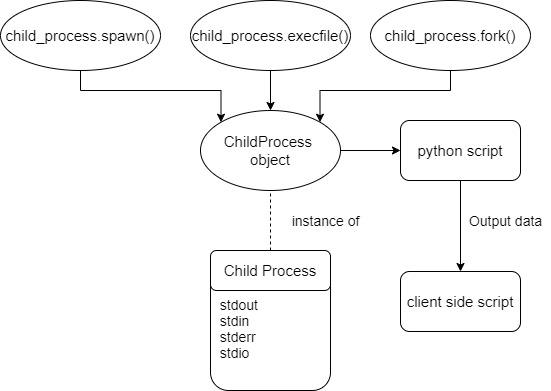
\includegraphics[width=4in]{capture_spawn.jpg}
		\end{center}
	\caption{Handling multiple requests}
	\end{figure}
\section{Implementation}
The android app has been prepared using Android Studio and the Nodejs Server is used for storing the data and running the script for detection of flood images.

\subsection{Frontend}

	\begin{figure}[h!]
		\begin{center}
		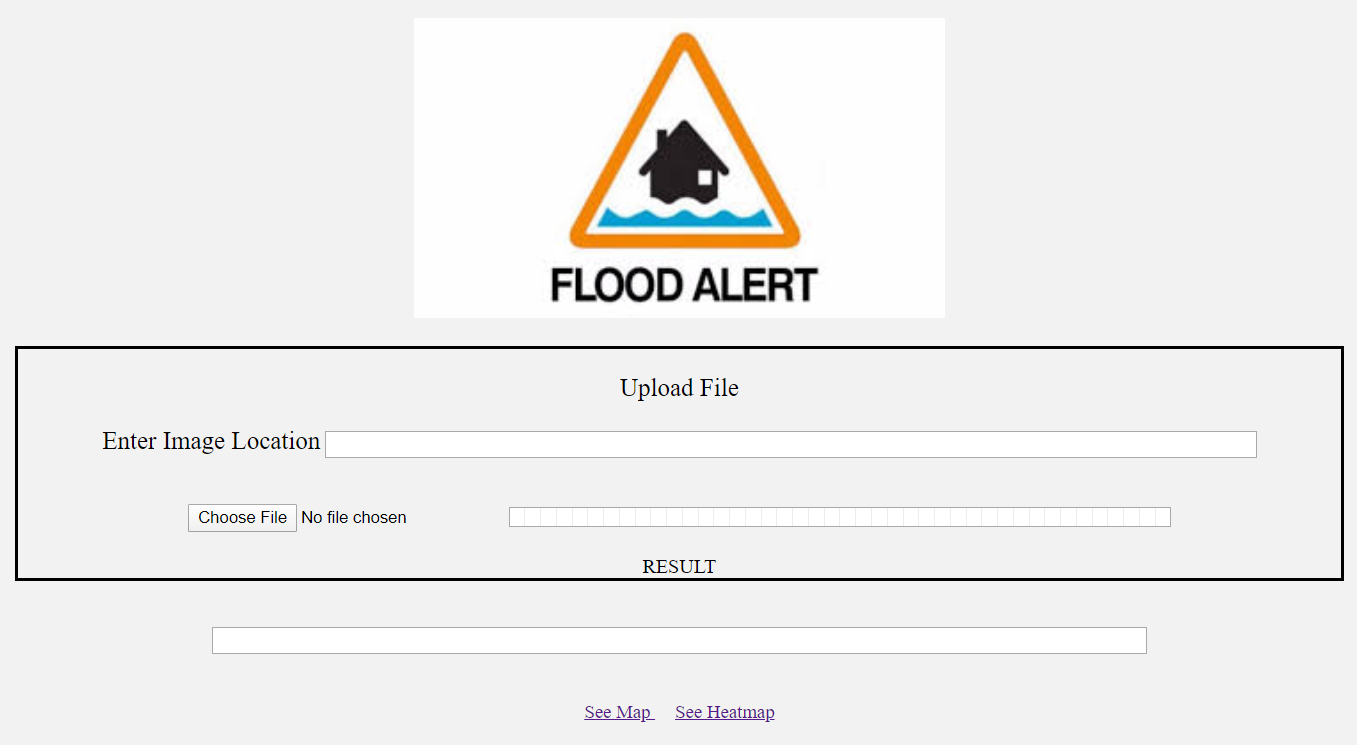
\includegraphics[width=4in]{Capture 1.png}
		\end{center}
	\caption{UI design}
	\end{figure}
	\begin{enumerate}
	\item For Uploading image to server:
		\begin{enumerate}[Step 1:] 
		\item Image upload to the node server.
		\item  If successful upload then call the python script predict.py.
		\item Return the result as water percentage and provided to the user. 		
		\end{enumerate}
	\item To view affected areas on map (or heatmap).
		\begin{enumerate}[Step 1:] 
		\item Enter the desired area to be viewed (city).
		\item If valid city, call python script GeoLocation.py which returns the coordinates of each image uploaded to the server in that city.
		\item A list of coordinates are returned which are indicated as markers on the map.		
		\end{enumerate}
	\item To click an image on map:
		\begin{enumerate}[Step 1:] 
		\item Click on the marker indicated on the map.
		\item Call the python script extract\_images.py.
		\item Returns the pathname of the image file in the server.
		\item Image displayed in an infobox.		
		\end{enumerate}
	\end{enumerate}

\subsection{Backend}
The Express Server is used as the Backend module framework.Once the image file reaches the server endpoint, it is parsed using the formidable module to extract the path name of the file.A child process is spawned from the Node Server and a python script is invoked from it.The path of the image file is passed as a parameter to the Python script.The Python script performs image binarization on the uploaded image and returns the desired output  to the Node Server which inturn is sent back as a response to the client and displayed on the screen.

\subsection{Deep learning approach}
The implementation of the backend code is done in python. There are two python scripts:
	\begin{enumerate}
		\item For training using the available datasets.
		\item Prediction of images provided by rescue personnel.
	\end{enumerate}
\subsubsection{Training dataset}
	\begin{enumerate}
	\item \textbf {Generation of flood-water training samples:} To 		generate flood-water training samples, several flood Images are collected from www.google.com with the keyword pattern: “ Flood”, for example, “Orissa Flood”, “Mumbai Flood” etc.\\
Then we manually cropped only the flood water regions, those were used further for training samples generation. 
\item \textbf {Generation of non-water training samples:} To generate non-water samples, various keywords were used to download images, a few of them being: animals, cars, paintings, face, flowers, house, text, trees etc. However, we excluded any image having some water presence.
	\end{enumerate}
	\begin{figure}[h!]
		\begin{center}
		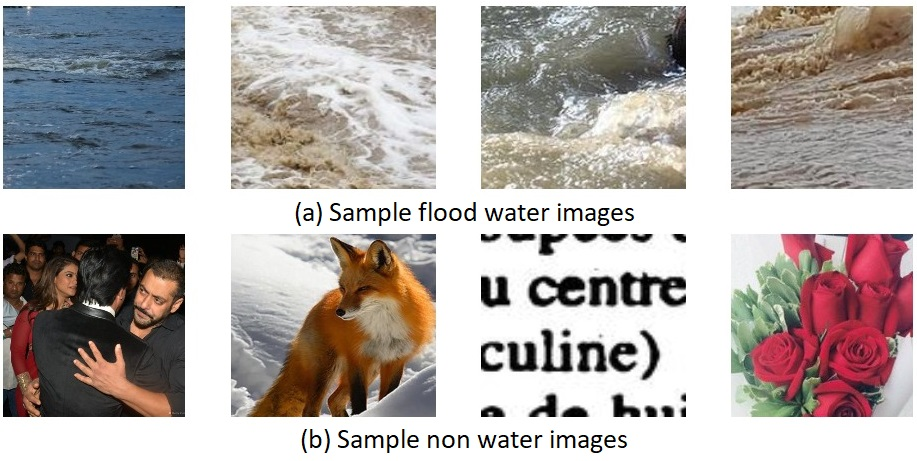
\includegraphics[width=4in]{training_data.jpg}
		\end{center}
	\caption{Sample training data}
	\end{figure}
\subsubsection{Flood-water-detector model}
Convolutional neural networks are a class of deep, feed-forward artificial neural networks which are widely used in computer vision applications. CNNs use a variation of multilayer perceptrons. They use a special architecture which is particularly well adapted to classify images. It uses three basic ideas: local receptive fields, shared weights, and pooling. CNNs are translational invariant. The CNNs are also used in the field of speech recognition and natural language processing. In this work, we propose a CNN-based flood-water-detector model.\\
We use 2 approaches to create model:
	\begin{enumerate}
	\item Creating our own model for training and prediction.
	\item Using transfer learning and performing layer unfreezing.
	\end{enumerate}
The proposed CNN model is trained using two different kinds of image samples: \\\textbf{(i) flood-water and (ii) non-water}\\[0.5cm]
 We use a training sample dimension of $48*48*3$. We run a non overlapping window of size $48*48*3$ over the entire set of images ( both water and non water) and thus create a dataset of images of size $48*48*3$ The window size $48*48*3$ is moved from left to right and top to bottom, and the image under the window is cropped to produce several image patches.  A total of 54K samples are generated out of flood-water samples and non-water samples. Out of these 50K samples we use 21K samples for training the model and 9K samples are used for the validation of the CNN model. The rest 20K samples are kept for testing of the flood-water-detector .
 
	\begin{figure}[h!]
		\begin{center}		
		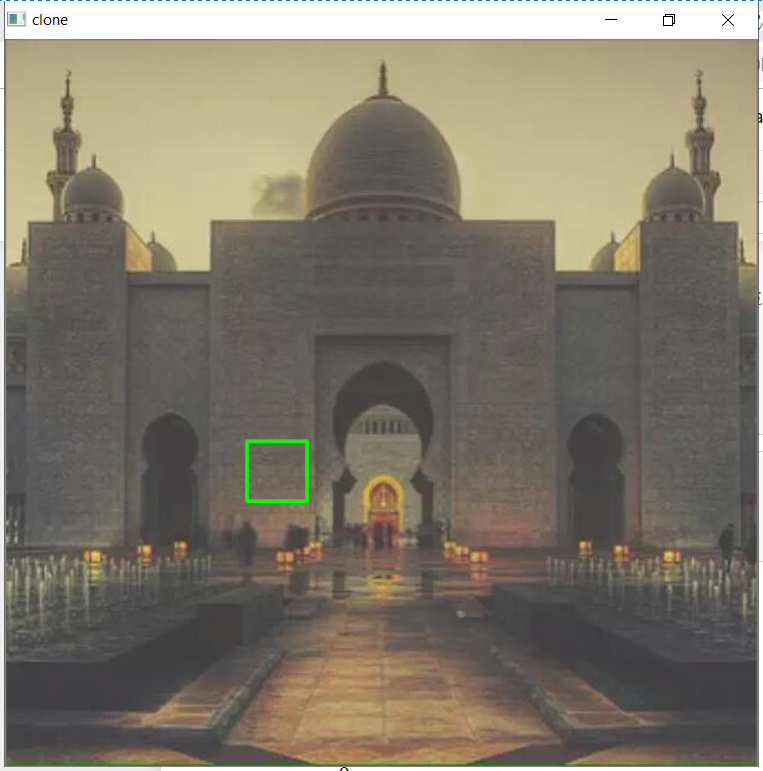
\includegraphics[width=3in]{pasted image 0.png}
	\caption{Green rectangle $\rightarrow$ window of size $48*48*3$ sliding throughout the image.}
	\end{center}
	\end{figure}

\begin{center}
\begin{figure}[h!]
  
    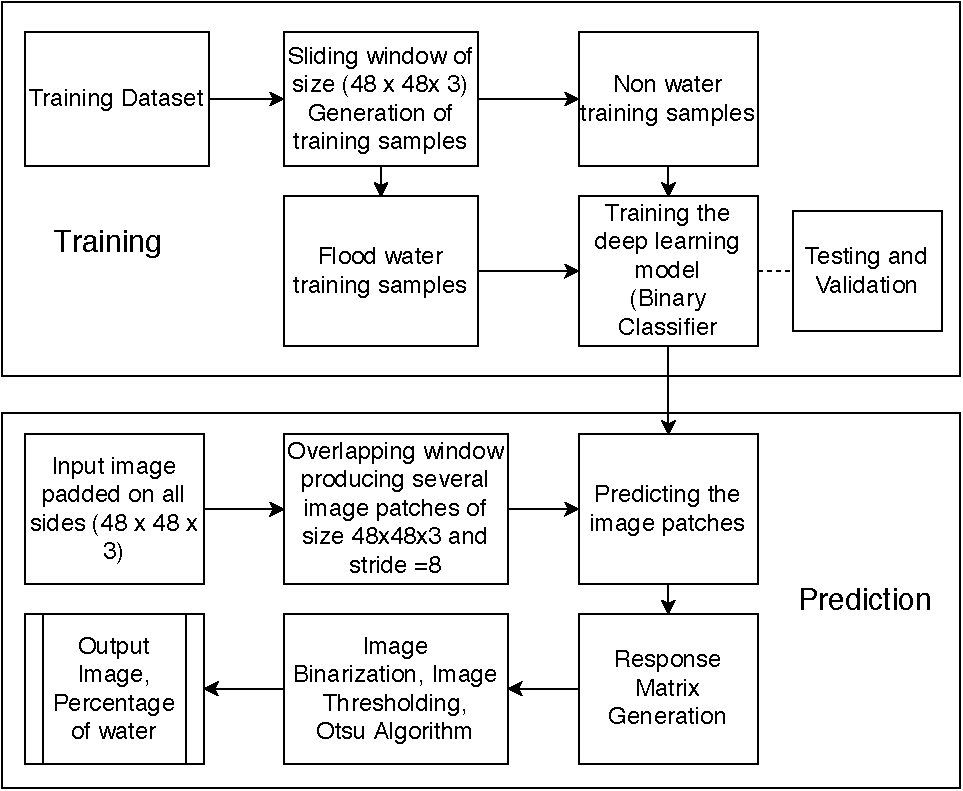
\includegraphics[page=1,width=1\textwidth]{flowchart.pdf}\hspace*{5\textwidth}
  \caption{Flowchart}
\end{figure}
\end{center}

\begin{enumerate}
\item \textbf {Architecture of own model:}
The CNN architecture that we used consists of four convolution layers, two fully connected layer (FC) and one softmax layer. Each convolution layer is followed by a dropout layer which is again followed by a rectification layer (ReLU). The output is fed into the max pooling layer which again is fed into the next block of layers. The softmax layer is required for classification.
\newpage
	\begin{table}[h!]
	\begin{tabular}{|c|c|c|c|c|}
	\hline
	Serial & Layer & Filter & Number of & Output \\ 
	No. & Type & Dimension & Filters & Dimension \\ \hline
	1 & Input & - & - & $48*48*3$ \\ \hline
	2 & Convolution + Dropout (0.2)& $3*3*3$ & 64 & $48*48*64$ \\
	3 & Max Pooling& $2*2$ & - & $24*24*64$ \\ \hline 
	4 & Convolution + Dropout (0.2)& $3*3*3$ & 128 & $24*24*128$ \\
	5 & Max Pooling& $2*2$ & - & $12*12*128$ \\ \hline 
	6 & Convolution + Dropout (0.2)& $3*3*3$ & 256 & $12*12*256$ \\
	7 & Max Pooling& $2*2$ & - & $6*6*256$ \\ \hline 
	8 & Convolution +  Dropout (0.2)& $3*3*3$ & 512 & $6*6*512$ \\
	9 & Max Pooling& $2*2$ & - & $3*3*512$ \\ \hline 
	10 & Fully Connected (64)+ Dropout (0.2) & - & - & $1*1*64$ \\ \hline
	11 & Fully Connected (2) & - & - & $1*1*2$ \\
	12 & Softmax (Output) & - & - & $1*1*2$ \\ \hline
	\end{tabular}
	\begin{center}
Model architecture\\
\end{center}
	\end{table}
	
Total params: 4,980,482\\
Trainable params: 4,980,482\\
Non-trainable params: 0\\[1cm]
Training Accuracy Achieved: 88.74\%\\
Validation Accuracy: 88.23\%\\

\item \textbf {Transfer learning approach:}
With transfer learning, instead of starting the learning process from scratch, we start from patterns that have been learned when solving a different problem.  In computer vision, transfer learning is usually expressed through the use of pre-trained models. A pre-trained model is a model that was trained on a large benchmark dataset to solve a problem similar to the one that we want to solve. Due to the computational cost of training such models, it is common practice to import and use the models: VGG, Inception, MobileNet.\\[1cm]
In our problem, we use the VGG19 pretrained model.
In VGG19, the image input size is $224*224*3$. However, as discussed earlier, the model is presented with an input image of size $48*48*3$. This is made possible because in transfer learning only the layer weights (i.e the parameters) are loaded which are independent of the size of the input image. \\[1cm]
While using a pre-trained model the original classifier has to be removed, and a new classifier has to be added that fits specified purposes. Finally the model has to be fine tuned according to one of the three strategies:\\
There are 3 ways of using transfer learning:
\begin{enumerate}
\item Freezing the entire convolutional base.
\item Train some layers and leave the others frozen.
\item We use the architecture of the pre-trained model and train it according to our dataset.
\end{enumerate}
All these 3 methods were experimented with.
	\begin{figure}[h!]
		\begin{center}		
		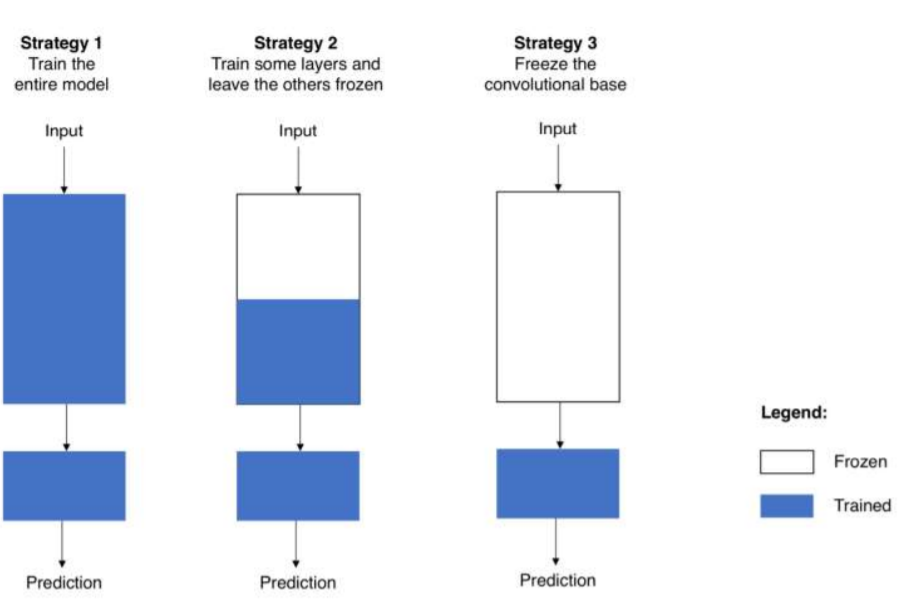
\includegraphics[width=3in]{pasted image 0 (2).png}
	\caption{Strategies related to transfer learning}
		\end{center}
	\end{figure}

Architecture of VGG19 model and the output shapes:\\
	\begin{tabular}{|c|c|c|c|c|}
	\hline
	Serial & Layer & Filter & Number of & Output \\ 
	No. & Type & Dimension & Filters & Dimension \\ \hline
	1 & Input & - & - & $48*48*3$ \\ \hline
	2 & block1\_conv1 (Conv2D)& $3*3*3$ & 64 & $48*48*64$ \\
	2 & block1\_conv2 (Conv2D) & $3*3*3$ & 64 & $48*48*64$ \\
	3 & block1\_pool (MaxPooling2D)  & $2*2$ & - & $24*24*64$ \\ \hline 
	4 & block2\_conv1 & $3*3*3$ & 128 & $24*24*128$ \\
	4 & block2\_conv2 & $3*3*3$ & 128 & $24*24*128$ \\
	5 & block2\_pool (MaxPooling2D)& $2*2$ & - & $12*12*128$ \\ \hline 
	6 & block3\_conv1& $3*3*3$ & 256 & $12*12*256$ \\
	6 & block3\_conv2& $3*3*3$ & 256 & $12*12*256$ \\
	6 & block3\_conv3& $3*3*3$ & 256 & $12*12*256$ \\
	6 & block3\_conv4& $3*3*3$ & 256 & $12*12*256$ \\
	7 & block3\_pool (MaxPooling2D) & $2*2$ & - & $6*6*256$ \\ \hline 
	8 & block4\_conv1 & $3*3*3$ & 512 & $6*6*512$ \\
	8 & block4\_conv2 & $3*3*3$ & 512 & $6*6*512$ \\
	8 & block4\_conv3 & $3*3*3$ & 512 & $6*6*512$ \\
	8 & block4\_conv4 & $3*3*3$ & 512 & $6*6*512$ \\
	9 & block4\_pool (MaxPooling2D)& $2*2$ & - & $3*3*512$ \\ \hline 
	8 & block5\_conv1 & $3*3*3$ & 512 & $3*3*512$ \\
	8 & block5\_conv2 & $3*3*3$ & 512 & $3*3*512$ \\
	8 & block5\_conv3 & $3*3*3$ & 512 & $3*3*512$ \\
	8 & block5\_conv4 & $3*3*3$ & 512 & $3*3*512$ \\
	9 & block5\_pool (MaxPooling2D)& $2*2$ & - & $1*1*512$ \\ \hline 
	10 & Fully Connected (64)& - & - & $1*1*64$ \\ \hline
	11 & Fully Connected (2) & - & - & $1*1*2$ \\
	12 & Softmax (Output) & - & - & $1*1*2$ \\ \hline
	\end{tabular}
	\begin{center}
	Model architecture\\
	\end{center}
Total parameters:  20,090,306\\[1cm]
The three approaches taken:\\
	\begin{enumerate}
	\item Using the Convolution base: Usually done when the dataset is very small and/or computation power is limited. All layers are frozen.\\	
Model summary:\\[0.5cm]
	\begin{tabular}{|c|c|c|}
	\hline
	Layer Type & Output Shape & Param\#\\ \hline
	model (Model) & (None, 512) & 20024384\\ \hline
	dense\_2 (Dense) & (None, 128) & 65664\\ \hline
	dense\_3 (Dense) & (None, 2) & 258\\ \hline
	\end{tabular}
\\[0.5cm]
Total params: 20,090,306\\
Trainable params: 0\\
Non-trainable params: 20,090,306\\[1cm]\\
Model test:\\[0.5cm]
	\begin{tabular}{|c|c|c|c|}
	\hline
Class Label & Precision & Recall & F - score\\ \hline
0 (Non water) & 0.99  & 0.98 & 0.99\\ \hline
1 (water) & 0.89 & 0.89 & 0.89\\ \hline
	\end{tabular}
\\
accuracy: 94\%\\
	\item Here, we played with the dichotomy by choosing how much we want to adjust the weights of the network. The number of layers that need to be frozen and those which need to be unfrozen depend upon the size of the dataset and its similarity to the dataset in which our pre-trained model was trained.
	\begin{figure}[h!]	
		\begin{center}
		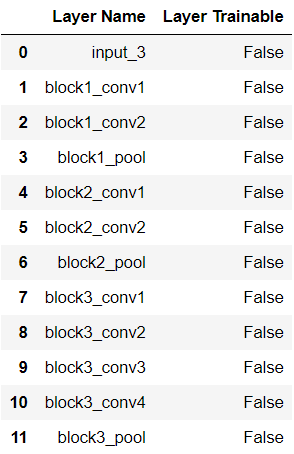
\includegraphics[width=2in]{pasted image 0 (3).png}
		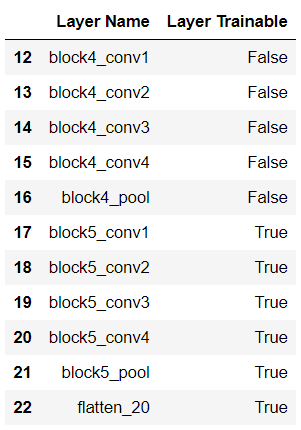
\includegraphics[width=2in, height=3.143in]{pasted image 0 (10).png}
		\end{center}
	\caption{Layer description}
	\end{figure}		
\newline
True $\rightarrow$ Layers Unfrozen \\
False $\rightarrow$ Layers Frozen\\[0.5cm]
\clearpage
Model summary:\\[1cm]
	\begin{tabular}{|c|c|c|}
	\hline
Layer Type & Output Shape & Param\#\\ \hline
model\_19 (Model) & (None, 512) & 20024384\\ \hline
dense\_40 (Dense) & (None, 128) & 65664\\ \hline
dense\_41 (Dense) & (None, 2) & 258\\ \hline
	\end{tabular}
\\[0.5cm]
Total params: 20,090,306\\
Trainable params: 9,505,154\\
Non-trainable params: 10,585,152\\[1cm]\\
Model test:\\[0.5cm]
	\begin{tabular}{|c|c|c|c|}
\hline
Class Label & Precision & Recall & F - score\\ \hline
0 (Non water) & 0.99  & 0.99 & 0.99\\ \hline
1 (water) & 0.91 & 0.89 & 0.90\\ \hline
	\end{tabular}
\\
accuracy: 97.7\%\\
\item Unfreezing all the layers and just using the architecture to train the model. However, it might lead to overfitting. Can be used only if the dataset is large enough.
Model summary:\\[1cm]
\begin{tabular}{|c|c|c|}
\hline
Layer Type & Output Shape & Param\#\\ \hline
model\_19 (Model) & (None, 512) & 20024384\\ \hline
dense\_40 (Dense) & (None, 128) & 65664\\ \hline
dense\_41 (Dense) & (None, 2) & 258\\ \hline
\end{tabular}
\\[0.5cm]
Total params: 20,090,306\\
Trainable params: 20,090,306\\
Non-trainable params: 0\\[1cm]\\
Model test:\\[0.5cm]
\begin{tabular}{|c|c|c|c|}
\hline
Class Label & Precision & Recall & F - score\\ \hline
0 (Non water) & 0.99  & 0.98 & 0.99\\ \hline
1 (water) & 0.89 & 0.95 & 0.92\\ \hline
\end{tabular}
\\
accuracy: 98.2\%\\[0.5cm]\\
Comparative Study:
\begin{enumerate}
\item The VGG pretrained model performed better than the model created as it is a deeper network and is one of the best models for image classification.
\item Training the entire model leads to overfitting as there is less amount of data as well as the class imbalance problem. (Less data in water image class).
\item Freezing the entire convolution base works well as the data is very much similar to the benchmark data used in the pretrained model.
\end{enumerate}
\end{enumerate}
\end{enumerate}
\subsubsection{Response matrix generation (heatmap) and flood region identification}
	\begin{enumerate}
\item 	Response matrix generation: We use an overlapping sliding window approach to generate the response matrix for the input image. The size of the window is $48*48$ and its stride is 8 pixels (both vertical and horizontal) . As a preprocessing step, the input image is zero padded in all the sides of the images. 48 zeros are padded on the four sides of the image under test. These padded elements are discarded later to obtain the final response matrix.\\
Steps for Response Matrix Generation:
		\begin{enumerate}
		\item A Matrix named mask is prepared of the same dimensions of the input image (only 1 channel) $(48*48*1)$
		\item Each image patch $(48*48*3)$ is fed to the flood-water-detector model. The output is a prediction of value 1 (water) or 0 (non water).
		\item This value is added to all $48*48$  cells in the response matrix mask.
		\end{enumerate}
Algorithm:\\
$$mask[y:y + winW, x:x + winH] = mask[y:y + winW, x:x + winH]+np.full((48,48), y\_pred)$$
where,\\
$winW = winH =48$\\
	\begin{equation}
	y\_pred =
		\begin{cases}
      	0, & \text{if}\ image patch = non water \\
      	1, & \text{if}\ image patch = water \\
    	\end{cases}
	\end{equation}
\item Flood region identification: First the response matrix is divided by the maximum value in the response matrix . Then we convert the value in the matrix mask to 0 or 255 depending upon a threshold:
$\displaystyle{mask[i,j]=\frac{mask[i,j]}{maxval}}$
	\begin{equation}
	img[i,j] =
		\begin{cases}
      	0, & \text{if}\ mask[i,j] <= T \\
      	1, & \text{if}\ mask[i,j] > T\\
    	\end{cases}
	\end{equation}
where,
$T \rightarrow Threshold$\\
$0<T<1$\\
$maxval\rightarrow \text{Maximum value present in matrix mask}$\\
	\begin{figure}[h!]
	\begin{subfigure}{.5\textwidth}
	\begin{center}
		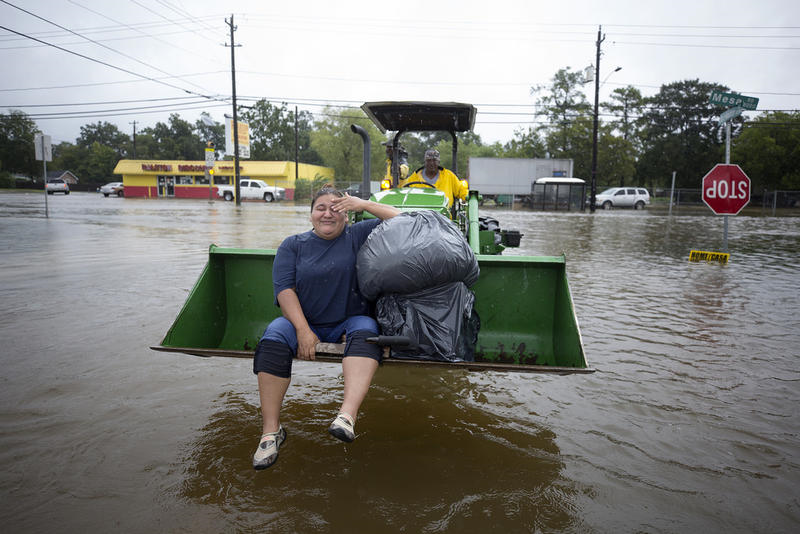
\includegraphics[width=2in]{pasted image 0 (4).png}
	\end{center}
	\caption{ Input image}
	\end{subfigure}
	\begin{subfigure}{.5\textwidth}
	\begin{center}
		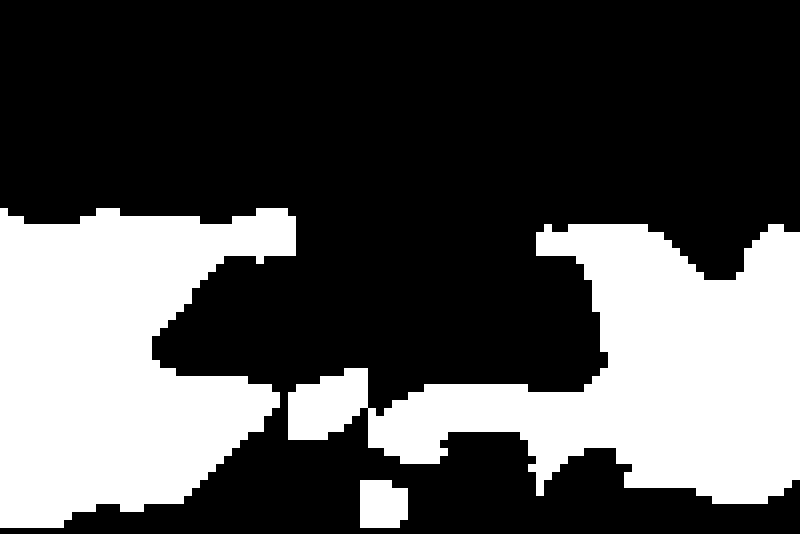
\includegraphics[width=2in]{pasted image 0 (5).png}
	\end{center}
	\caption{Flood region identification}
	\end{subfigure}
	\begin{subfigure}{.5\textwidth}
	\begin{center}
		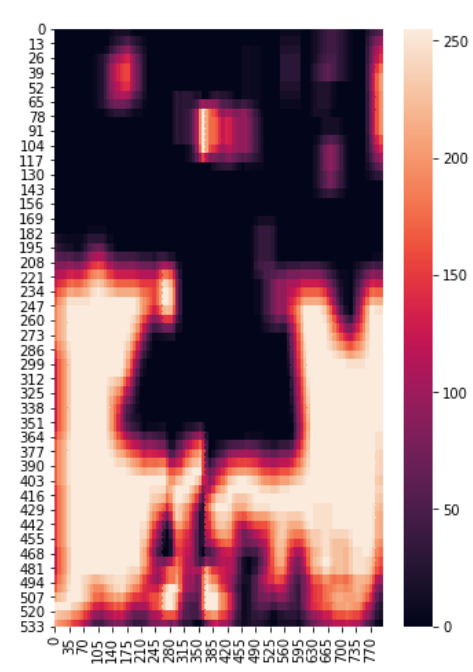
\includegraphics[width=2in,height = 1.5in]{pasted image 0 (6).png}
	\end{center}
	\caption{Heatmap (response matrix)}
	\end{subfigure}
	\caption{Input image \#1 and processing}
	\end{figure}
	\\[1cm]
	\begin{figure}[h!]
	\begin{subfigure}{.5\textwidth}
	\begin{center}
		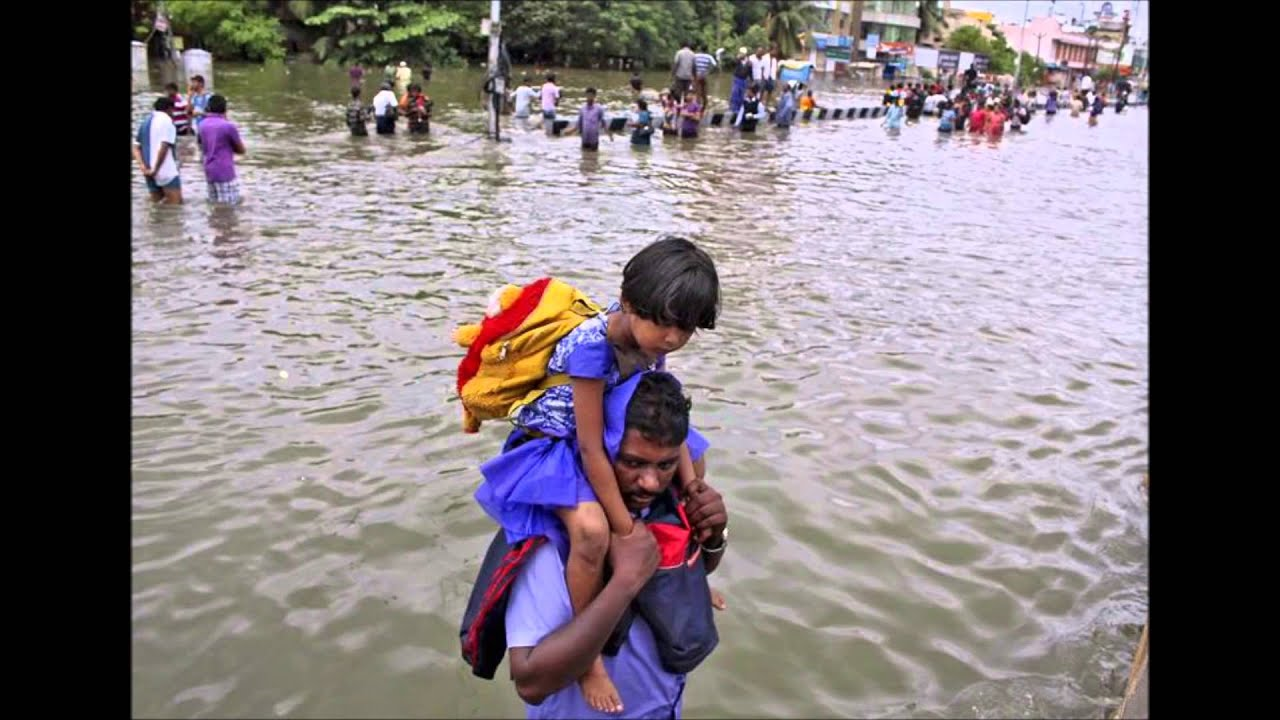
\includegraphics[width=2in]{pasted image 0 (7).png}
	\end{center}
	\caption{ Input image}
	\end{subfigure}
	\begin{subfigure}{.5\textwidth}
	\begin{center}
		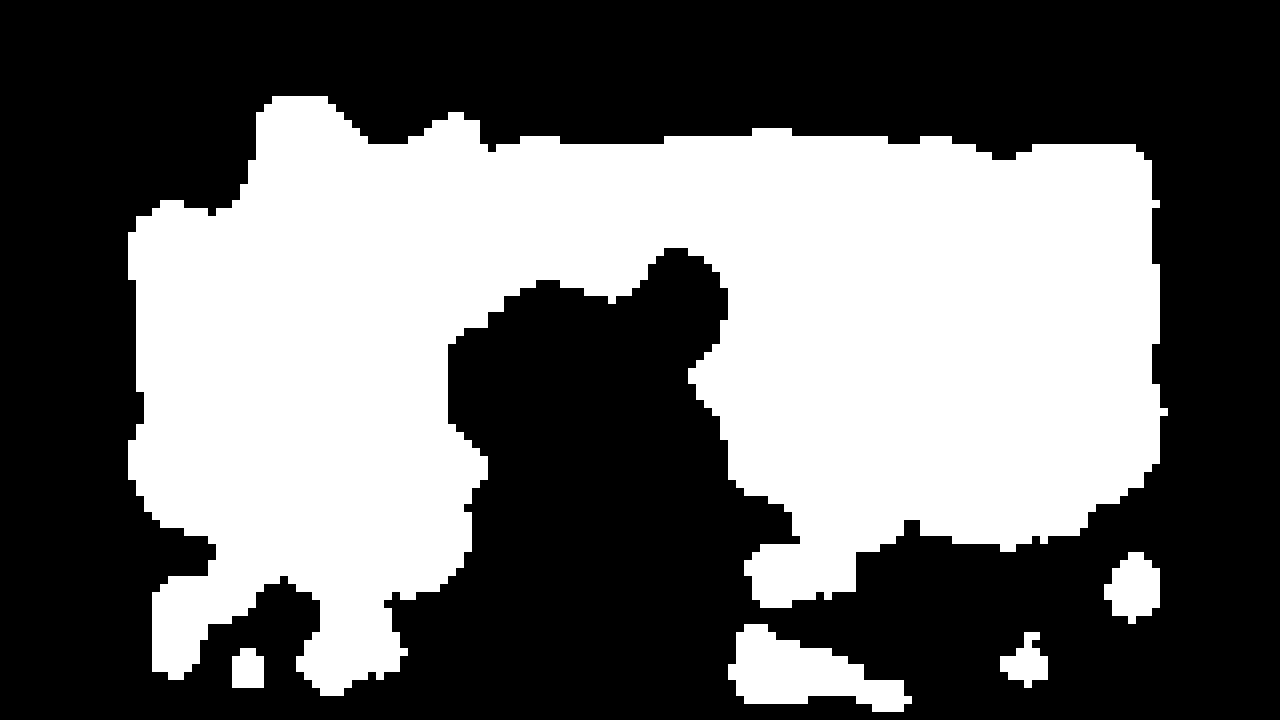
\includegraphics[width=2in]{pasted image 0 (8).png}
	\end{center}
	\caption{Flood region identification}
	\end{subfigure}
	\caption{Input image \#2 and processing}
	\end{figure}		

We also used the Otsu Algorithm for the image binarization.
Otsu’s algorithm is a simple and popular thresholding method for image binarization.The algorithm divides the image histogram into two classes, by using a threshold such that the in-class variability is very small. This way, each class will be as compact as possible. \\\\
Formally, a function g(x, y) can be defined over every pixel value of the original image f(x, y) that defines the new threshold image.\\
	\begin{equation}
	g(x, y)  =
		\begin{cases}
      	0, & \text{if}\ x<T \\
      	1, & \text{if}\ x \geq T \\
    	\end{cases}
	\end{equation}
where,
$T \rightarrow Threshold$\\
\item Region covered by water: After the image binarization, the percentage of image covered by water is calculated as follows:\\
$\displaystyle{\text{Percentage of image covered by water} = \frac{\text{No. of water pixel}}{\text{Total no. of pixels}}*100}$
\end{enumerate}
\section{Simulation}
In the absence of real dataset (images from flood affected locations) we simulated the data by scraping images of major flood havocs in recent years in cities such as Mumbai, Chennai, etc.\\
\subsection{Web scraping}
Scraping images from google requires the use of certain libraries like BeautifulSoup for pulling data out of HTML and XML files.\\
Also, we need to use \textbf{Selenium} webdriver Python API to emulate human browsing the website on the web browser (Chrome) and scroll down till the end of the album page. Once all the thumbnails are loaded on the page, the source code is parsed to identify the specific HTML tags with the links to the image display page.\\
\textbf{Selenium} is a tool to automate browsers. It’s primarily used for testing but is also very useful for web scraping. We need the suitable webdriver to perform this operation.
Steps for web scraping images:\\
	\begin{enumerate}
	\item The search term (e.g. “Mumbai Floods”) and the number of images (e.g. 500) need to be entered.
	\item An automated web browser with the given search term is opened and all the google images are loaded.
	\item The browser automatically starts to scroll down one-page height at a time until the end of the page has been reached and thus, loads all the thumbnails.
	\item We use “css-selectors” to get the relevant elements from the page i.e all the image links. 
	\item Following this, the automated web browser tries to click every thumbnail (img.click()) such that it can get the real image behind it.
	\item A directory is created to save all the images. 
	\end{enumerate}
	\begin{figure}[h!]	
		\begin{center}
		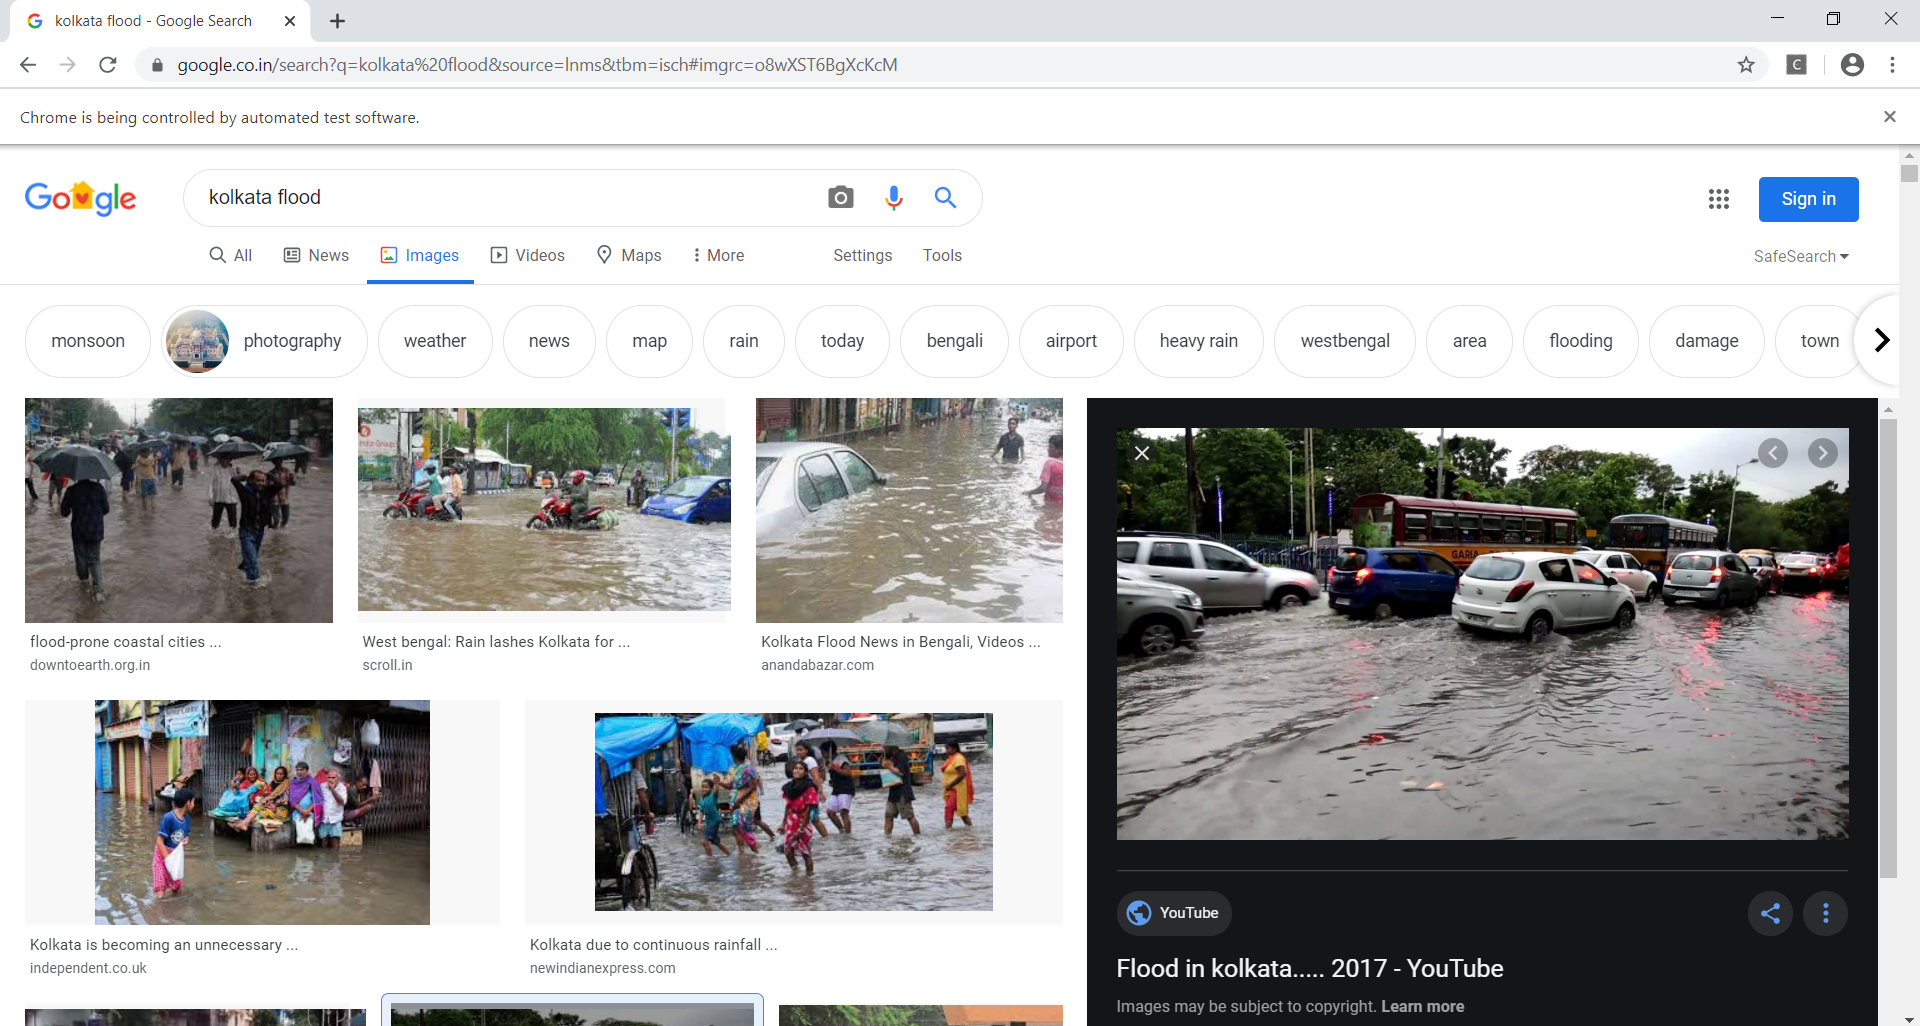
\includegraphics[width=4in]{Capture 2.png}
		\end{center}
	\caption{Web scraping using Selenium}
	\end{figure}

\subsection{Assigning coordinates to scrapped images}
Images scrapped from google do not contain geolocations i.e latitude and longitude (location) of the image. Thus in order to simulate a real calamity scenario (flood) we needed to assign coordinates to the images. This enabled us to plot them on the map.\\
In order to assign coordinates, the metadata of the image needed to be changed. Metadata of the image containing its coordinates is in the form of a dictionary as follows:\\
\begin{lstlisting}
{
    'GPSLatitudeRef': 'N',
    'GPSLatitude': ((36, 1), (7, 1), (5263, 100)),
    'GPSLongitudeRef': 'W',
    'GPSLongitude': ((115, 1), (8, 1), (5789, 100)),
    ...
}
\end{lstlisting}
We edited this dictionary and inserted our sets of coordinates to all the scrapped images.\\ 
\\\textbf{Algorithm for selecting coordinates:}\\
In order to simulate a real world scenario, we identified certain regions in cities that are low lying areas or are prone to floods. Example in Mumbai the areas of Andheri, Kurla, Sion, Juhu, Santacruz, etc were identified.\\
Coordinates of these locations were taken as cluster centres.
Each cluster centre is assigned a scrapped image and other images are distributed randomly to each of the clusters. Each cluster has a certain lower limit of number of images and an upper limit. 
Coordinates for the images were assigned randomly within 2km radius of the cluster centre.\\
This algorithm, is just for a simulated scenario and is based on ideal conditions\\
\\Algorithm for a particular cluster:
\begin{lstlisting}
cluster_size=random.randrange(10,150,1) # Lower limit =10, Upper limit=150
\end{lstlisting}
$covariance = $
$\begin{bmatrix}
1 & 0\\
0 & 1\\ 
\end{bmatrix}\text{\# covariance matrix}$

\begin{lstlisting}
x,y = np.random.multivariate_normal(cluster_center,covariance,cluster_size)
\end{lstlisting}
$img\_coodinates=cluster\_center - $
$\begin{bmatrix}
(2km) & (2km)
\end{bmatrix} +  ($
$\begin{bmatrix}
4Km 
\end{bmatrix} *$
$\begin{bmatrix}
x & y 
\end{bmatrix}$  )\\
where,\\
4 km is the diameter, 
$img\_coordinates$ are the newly assigned coordinates to scrapped images.

\section{Working with the simulated scenario}
After scraping the images, all the images which have flood water content less than a specified threshold are removed. The deep learning model is used to calculate the  water percentage which has been explained previously in detail.\\
All the images are plotted on terrain maps using the “ Maps JavaScript API “.\\
Markers are added for each image location.\\
Each marker has an on click event which opens the image in an infobox and its details.\\
	\begin{figure}[h!]	
		\begin{center}
		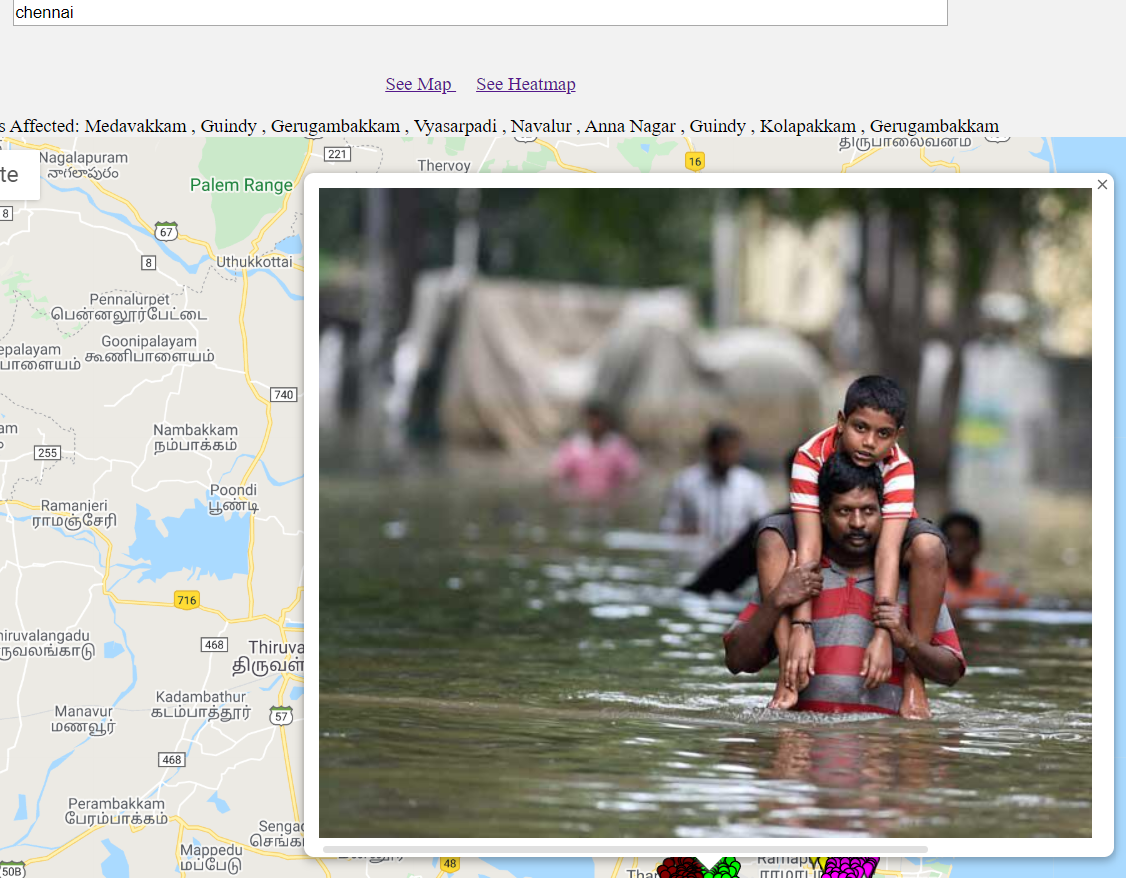
\includegraphics[width=4in]{Capture_infobox.png}
		\end{center}
	\caption{Image shown in infobox}
	\end{figure}

\subsection{Extraction of geo location from the metadata of an image}
Image metadata is text information pertaining to an image file that is embedded into the file.\\
Image metadata includes details relevant to the image itself as well as information about its production such as the GeoInfo.With photos stored in JPEG, JPG and many other file formats, the geotag information, storing camera location and sometimes heading, is typically embedded in the metadata, stored in Exchangeable image file format (Exif) or Extensible Metadata Platform (XMP) format.\\
GPSinfo is stored in metadata as:\\
	\begin{figure}[h!]	
		\begin{center}
		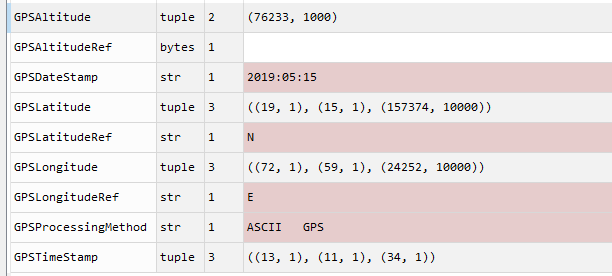
\includegraphics[width=4in]{pasted image 0 (9).png}
		\end{center}
	\caption{GPSinfo}
	\end{figure}	
\\This was used to place the marker in the Map to show the location of the flood affected image.\\
\subsection{Clustering}
We have specified the total number of cluster centres in our simulated scenario. However in reality the number of cluster centres is not specified. Thus the most suitable algorithm for clustering when the number of cluster centres and the shape of cluster is not known is the \textbf{DBSCAN algorithm}.\\
Density-based spatial clustering of applications with noise (DBSCAN) is a well-known data clustering algorithm that is commonly used in data mining and machine learning. Based on a set of points (let’s think in a bidimensional space as exemplified in the figure), DBSCAN groups together points that are close to each other based on a distance measurement and a minimum number of points. It also marks as outliers the points that are in low-density regions.\\
In our project where we have worked with geo coordinates, the parameters used for the DBSCAN algorithm are as follows:\\
\begin{lstlisting}
Distance measure = "Haversine"
Epsilon = 2 (km) / R
where R = 6373 km is the radius of earth
min_samples=2
\end{lstlisting}
Haversine distance measure is generally used for geo coordinates.\\
Epsilon is defined as the neighborhood around a data point i.e. if the distance between two points is lower or equal to ‘eps’ then they are considered as neighbors.\\
Algorithm used for DBSCAN is ‘ball tree’. This algorithm can avoid the need to calculate every possible distance. This is because the ball tree algorithm can use the triangular inequality theorem to reduce the number of candidates that need to be checked to find the nearest neighbours of a data point.\\
The DBSCAN algorithm gives the total number of estimated clusters. Using this we further implemented the \textbf{k - means algorithm} which gives the cluster centers.
	\begin{figure}[h!]	
		\begin{center}
		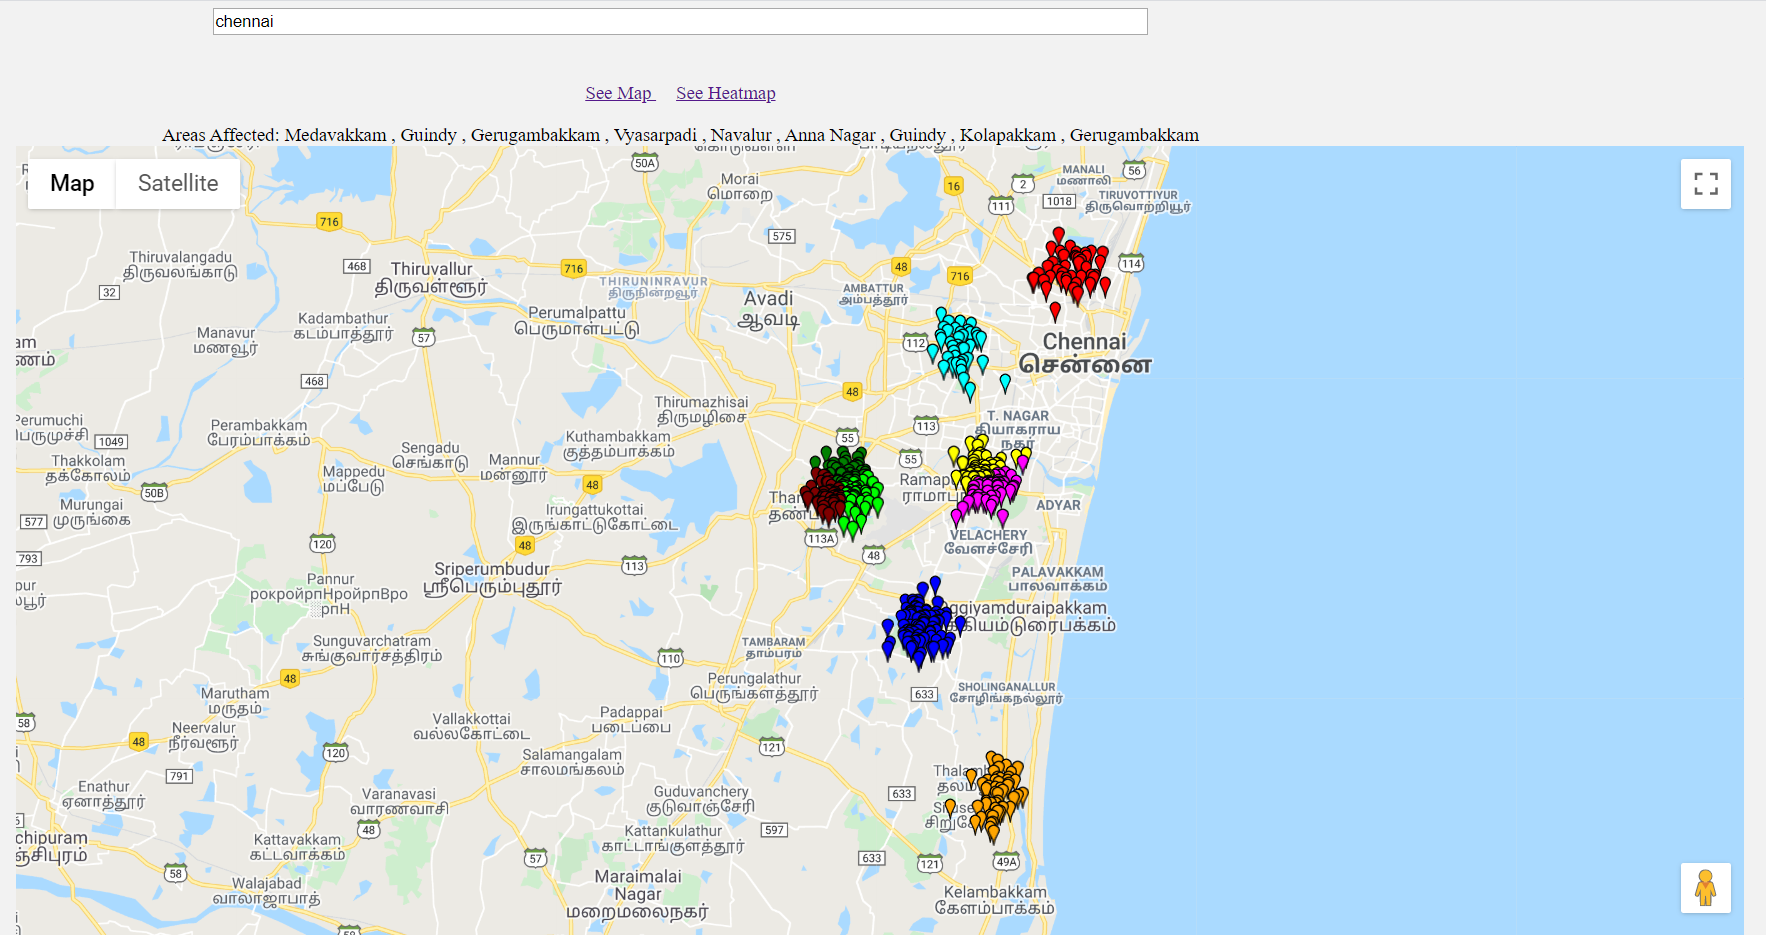
\includegraphics[width=4in]{Capture_chennai_cluster.png}
		\end{center}
	\caption{Various clusters of regions affected}
	\end{figure}	

\subsection{Generating heatmap}
A heatmap is a visualization used to depict the intensity of data at geographical points. When the Heatmap Layer is enabled, a colored overlay will appear on top of the map. By default, areas of higher intensity will be colored red, and areas of lower intensity will appear green.\\
Heatmap layer has been implemented in our project using the \textbf{google.maps.visualization} library provided by google maps.\\
	\begin{figure}[h!]	
		\begin{center}
		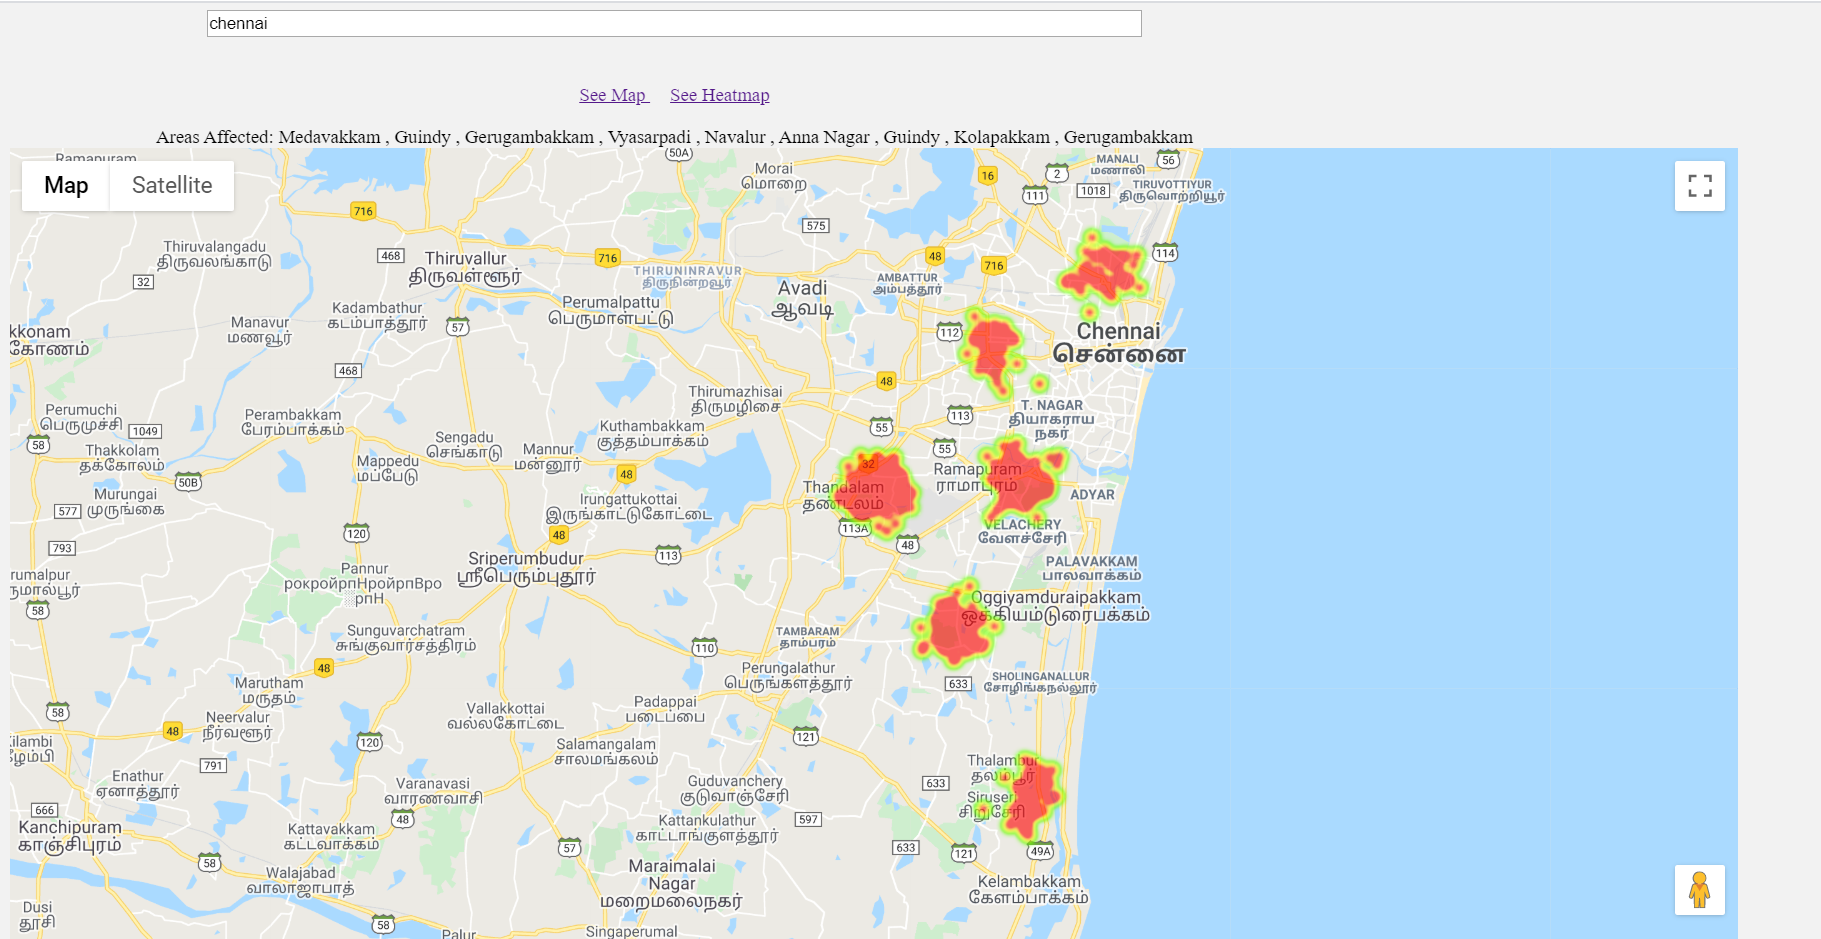
\includegraphics[width=4in]{Capture_chennai_heatmap_less_boundary.png}
		\end{center}
	\caption{Heatmap layer}
	\end{figure}
	
\subsection{Identifying affected localities}
Coordinates of the cluster centres can be retrieved after applying the k - means clustering on the set of images. These coordinates are helpful in order to find the center of the affected regions.\\
The set of cluster center coordinates are sent to the ‘The Geocoding API’ in order to get the address of the location.\\
The Geocoding API is a service that provides geocoding and reverse geocoding of addresses.\\
In this way we are able to retrieve the names of localities affected severely by floods.\\
	\begin{figure}[h!]	
		\begin{center}
		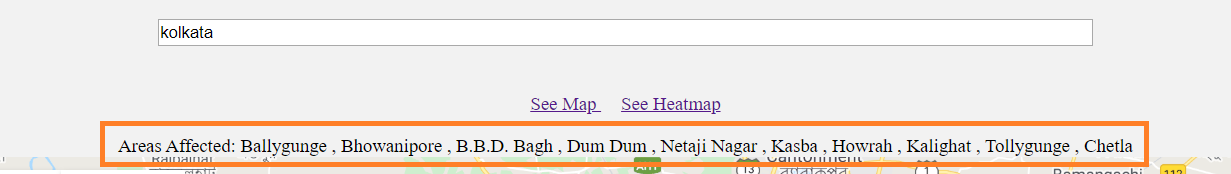
\includegraphics[width=4in]{Capture_kolkata_areas_affected.png}
		\end{center}
	\caption{Areas affected}
	\end{figure}
\subsection{Generating boundaries to identify “hotspots”}
By generating boundaries to the existing clusters of affected regions we can define certain regions as \textbf{“ hotspots ”} which can be immediately cordoned off so as to allow only rescue personnels, volunteers and health workers to access the area and provide relief support to the gravely affected residents of the area.\\
Boundaries are created with the Graham Scan algorithm which creates the smallest polygon encompassing all the coordinates.\\\\
\textbf{Convex hull}: For a given set of points S, the convex hull, denoted as CH(S), is the intersection of all convex regions containing S.\\
Graham scan algorithm is used to find the convex hull of a set of points.\\\\
\textbf{Graham scan algorithm:}\\
Choosing the bottommost point as an anchor (in case of multiple bottommost points, rightmost point is assumed among them), all other points are ordered based on the angles they form about this anchor. The hull is constructed by following this ordering, adding points for left hull turns and deleting for right turns.
	\begin{enumerate}
	\item P1 is considered as the bottom most point. From P1, lines are drawn to all other points.
	\item The vertices are sorted w.r.t the angles subtended (anti-clockwise) by their corresponding line segments with the horizontal line that passes through the bottommost point.(P1, P2,..., Pn).

	\item Further, the segment with the smallest angle is added as the first hull edge(P1, P2).
	\item P2, P3 is added as a hull edge. Following are the next steps.
	\end{enumerate}
\begin{algorithm}
\caption{Graham scan algorithm}
\begin{algorithmic}[1]
\State $ i \gets 2 $ , $ j \gets 3 $ , $ k \gets 4 $
\While {$ k \leq n $}
\If {$P_iP_jP_k \text{ is a right turn}$}
\While {$P_iP_jP_k \text{ is a right turn}$}
\State $\text{Remove edges } P_iP_j \text{ and } P_jP_k $
\State $\text{Add edge } P_iP_k$
\State $j = k$ , $k = k + 1$
\EndWhile
\Else 
\State $\text{ Add edge }P_jP_k \text{ as hull edge}$
\State $i = j$ , $j = k$ , $k = k + 1$
\EndIf
\EndWhile
\end{algorithmic}
\end{algorithm}
where, n is the number of input points.\\
The algorithm takes O(nLogn) time if we use a O(nLogn) sorting algorithm.\\
	\begin{figure}[h!]	
		\begin{center}
		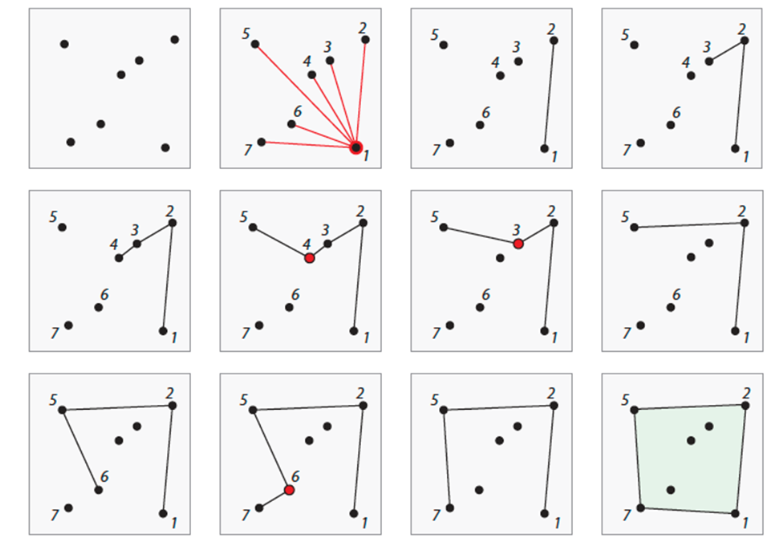
\includegraphics[width=4in]{Capture_graham_scan.png}
		\end{center}
	\caption{Graham scan algorithm}
	\end{figure}
		\begin{figure}[h!]	
		\begin{center}
		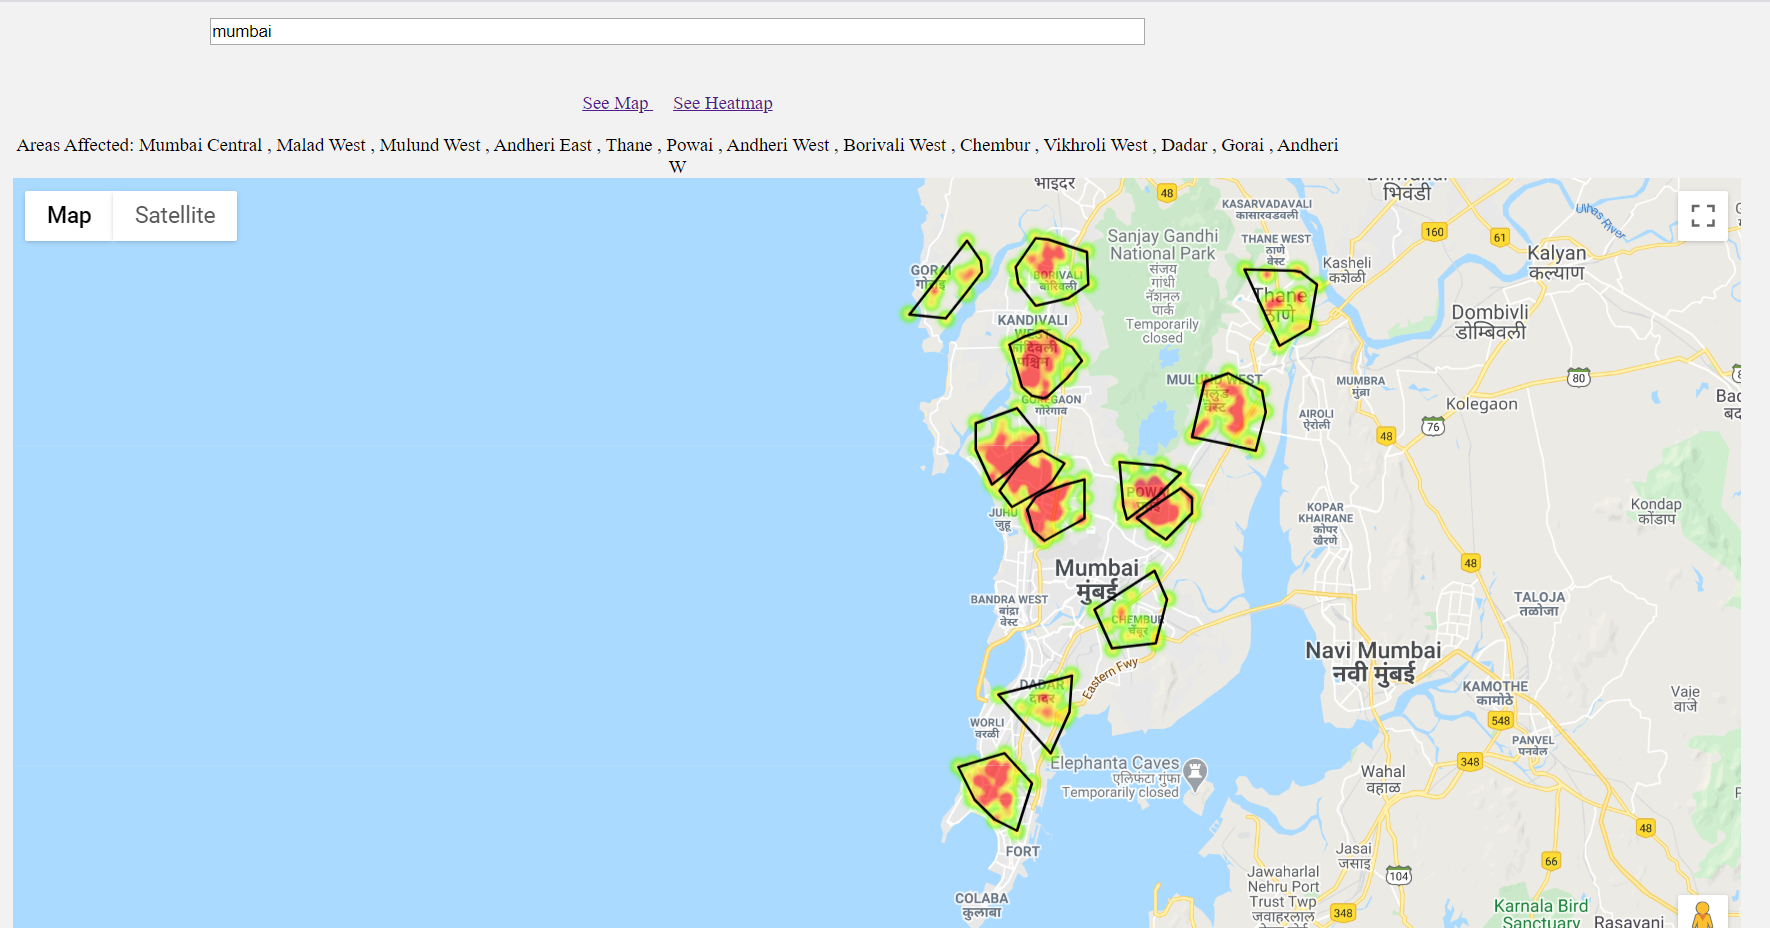
\includegraphics[width=4in]{Capture_mumbai_heatmap.png}
		\end{center}
	\caption{Generating heatmap and identifying hotspots}
	\end{figure}
\newpage
\section{Results}
\begin{enumerate}
\item The model developed is very accurate (~95\%) in detecting water and non water regions in the image.
\item The overlapped sliding window approach helps in effectively binarizing the image into water and non water regions.
\item The deep learning approach to calculate the percentage of flood water in the image effectively filters out unwanted and wrong images that have been uploaded to the application.
\item The images uploaded in the application would be readily available to the public and it would notify the people of regions affected by the calamity.
\item Citizens travelling across the city and public transport can be made cautious to restrain themselves from travelling to such disaster affected regions.
\item The localities identified as ‘ hotspots ‘ would quickly alert the rescue personnels and civic volunteers to carry out relief operations in those zones.

\end{enumerate}
\section{Future scope}
\begin{enumerate}
\item Over a period of time the data can be analyzed and certain flood prone “hotspots” can be identified which need robust infrastructure, road maintenance and \textbf{storm water drainage} facilities.
\item Strategic location of emergency shelter homes can be found out.
\item Such data would be very useful for municipal corporations and NDRF teams working during crisis periods.
\end{enumerate}
\section{Challenges}
\begin{enumerate}
\item The results obtained using the deep learning models had very good training accuracy as well as test accuracy. However, it performed moderately in image segmentation. Thus there is a need for performing other image segmentation and preprocessing     techniques and a comparative study between different techniques.
\item Certain portions in the water which have reflections or shadows, are treated as non water objects. There is scope for improvement in this aspect.
\item Only those images having locations in their metadata can be accepted by the application.
\item Deliberately manipulating image metadata and uploading fake images remains a challenge. 
\item To make the application useful, there must be general awareness among the public and eagerness to contribute towards the benefit of the society. 
\end{enumerate}
\bibliographystyle{apacite}
	
\bibliography{References}
https://developers.google.com/maps\\
https://towardsdatascience.com/image-scraping-with-python-a96feda8af2d
\\
https://towardsdatascience.com/a-comprehensive-hands-on-guide-to-transfer-learning-with-real-world-applications-in-deep-learning-212bf3b2f27a\\
https://medium.com/kansas-city-machine-learning-artificial-intelligen/an-introduction-to-transfer-learning-in-machine-learning-7efd104b6026\\
https://whatis.techtarget.com/definition/image-metadata\\
https://towardsdatascience.com/a-comprehensive-hands-on-guide-to-transfer-learning-with-real-world-applications-in-deep-learning-212bf3b2f27a
\\
https://medium.com/kansas-city-machine-learning-artificial-intelligen/an-introduction-to-transfer-learning-in-machine-learning-7efd104b6026
\\
https://whatis.techtarget.com/definition/image-metadata

%\cite{8882877}
%\cite{8075343}
%\cite{inproceedings}
%\cite{Chaudhary2019FLOODWATERLE}
\end{document}